%!TEX root = ../Demo.tex
\chapter{自动机状态转移图}

%%  接受{$\mathcal{L}$}=0*10*的自动机{\cite[fig 5-4]{book1}}

\begin{figure}[!htbp]
    \centering
    \begin{subfigure}[b]{0.35\textwidth}
        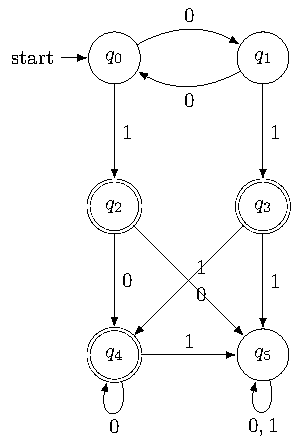
\includegraphics[width=\textwidth]{automaton_4_0}
        \caption{}
        \label{fig:DFA4_0}
    \end{subfigure}
    ~
    \begin{subfigure}[b]{0.35\textwidth}
        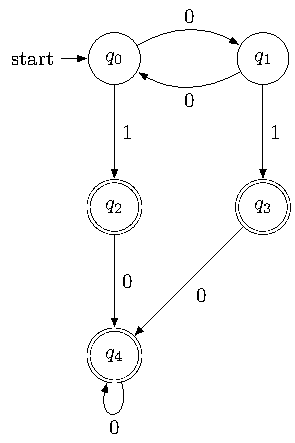
\includegraphics[width=\textwidth]{automaton_4_1}
        \caption{}
        \label{fig:DFA4_1}
    \end{subfigure}
    \\
    \begin{subfigure}[b]{0.35\textwidth}
        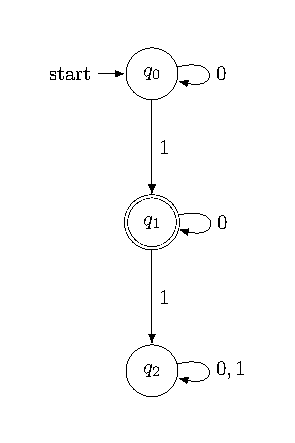
\includegraphics[width=\textwidth]{automaton_4_2}
        \caption{}
        \label{fig:DFA4_2}
    \end{subfigure}
    ~
    \begin{subfigure}[b]{0.35\textwidth}
        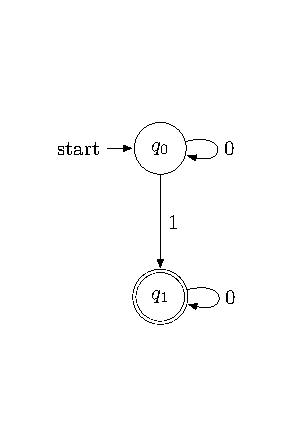
\includegraphics[width=\textwidth]{automaton_4_3}
        \caption{}
        \label{fig:DFA4_3}
    \end{subfigure}
    \caption{(a)接受{$\mathcal{L}$}=0*10*的自动机{\cite[fig 5-4]{book1}};  (b) 图(a)去除非 “final-reachable” 状态 {$q_5$}; (c) 与图(a) 的 $DFA$ 同构的含有陷阱状态的最小 $DFA$ ;(d) 与图(a) 的 $DFA$ 同构的不含陷阱状态的最小 $DFA$。}
    \label{fig:DFA4}
\end{figure}


\begin{figure}[!htbp]
  \centering
  \begin{subfigure}[b]{0.35\textwidth}
      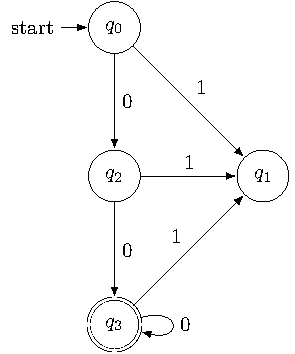
\includegraphics[width=\textwidth]{usefulf2-1}
      \caption{}
      \label{fig:usefulf2-1}
  \end{subfigure}
  ~
  \begin{subfigure}[b]{0.35\textwidth}
      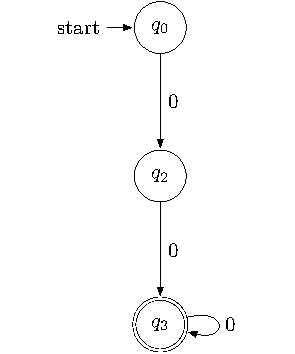
\includegraphics[width=\textwidth]{usefulf2-2}
      \caption{}
      \label{fig:usefulf2-2}
  \end{subfigure}
  \caption{(a)接受{$\mathcal{L}$}=000*的 DFA;  (b) 图(a)去除非 “final-reachable” 状态 {$q_1$}; }
  \label{fig:usefulf2-0}
\end{figure}


\begin{figure}[!htbp]
  \centering
  \begin{subfigure}[b]{0.6\textwidth}
      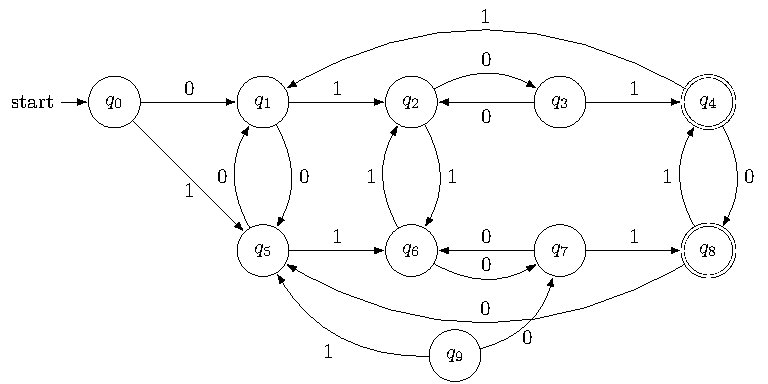
\includegraphics[width=\textwidth]{DFA11-0}
      \caption{}
      \label{fig:DFA11-0}
  \end{subfigure}
  \\
  \begin{subfigure}[b]{0.6\textwidth}
      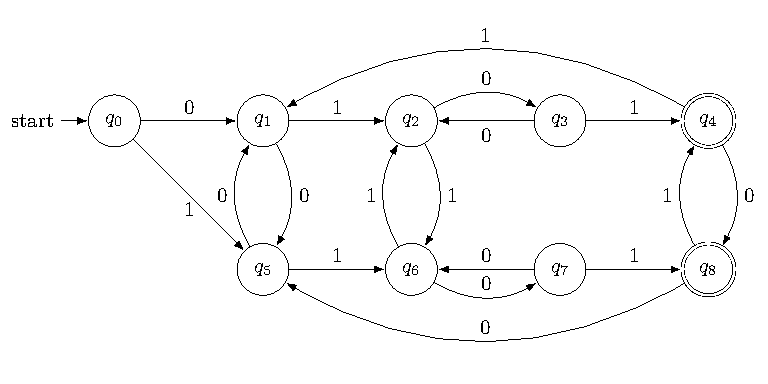
\includegraphics[width=\textwidth]{DFA11-1}
      \caption{}
      \label{fig:DFA11-1}
  \end{subfigure}
  \\
  \begin{subfigure}[b]{0.6\textwidth}
      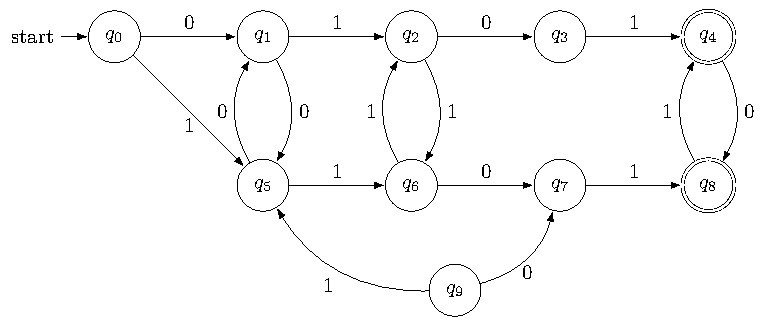
\includegraphics[width=\textwidth]{DFA11-2}
      \caption{}
      \label{fig:DFA11-2}
  \end{subfigure}
  \caption{(a)一个DFA;  (b) 图(a) 去除非 “start-reachable” 状态 {$q_9$};(c) 图(a)移除转移关系$T=\{(4 \times 1 \times 1),(8 \times 0 \times 5),(3 \times 0 \times 2),(7 \times 0 \times 6)\}$后的DFA。 }
  \label{fig:DFA11}
\end{figure}